\chapter{A tabela de avanço}\label{ch:g10:reaction-progress-table}
% ledger: use:NaN3-airbag
Numa batida de carro, uma almofada salta do volante e se enche de gás
numa fração de segundo, antes que a cabeça do motorista se mova para a
frente. O gás é produzido por uma \omterm{def:g7:chemical-reactions:reaction}{reação química}: uma pequena carga de
sólido, a azida de sódio no modelo clássico, se decompõe em sódio e
nitrogênio. O engenheiro precisa pôr sólido suficiente para encher a
almofada, mas não tanto que ela estoure, e nenhum \omterm{def:g7:chemical-reactions:reactant}{reagente} pode sobrar
para fazer mal aos passageiros. Quanto sólido dá quanto gás? Uma \omterm{def:g8:balanced-equations:equation}{equação
balanceada} dá as proporções; este capítulo as transforma numa ferramenta
de contabilidade que acompanha cada \omterm{def:g7:chemical-reactions:reactant}{reagente} e cada produto do começo ao
fim de uma reação.

\begin{recall}
Uma \omterm{def:g8:balanced-equations:equation}{equação balanceada} mantém o número de \omterm{def:g7:atoms-and-molecules:atom}{átomos} de cada elemento, e a
carga, iguais dos dois lados; os seus coeficientes dão as proporções em
que as espécies reagem (\cref{ch:g8:balanced-equations}). A \omterm{def:g10:the-mole:amount}{quantidade
de matéria} de uma espécie é $n = m/M$ para uma massa, $n = V/V_m$ para um
gás (com $V_m = \qty{24.1}{L/mol}$ a \qty{20}{\celsius} e à pressão
atmosférica normal) (\cref{ch:g10:the-mole}), e $n = c \times V$ para um
\omterm{def:g6:solutions-and-solubility:solute}{soluto} (\cref{ch:g10:concentration-and-dilution}).
\end{recall}

\begin{omfigure}
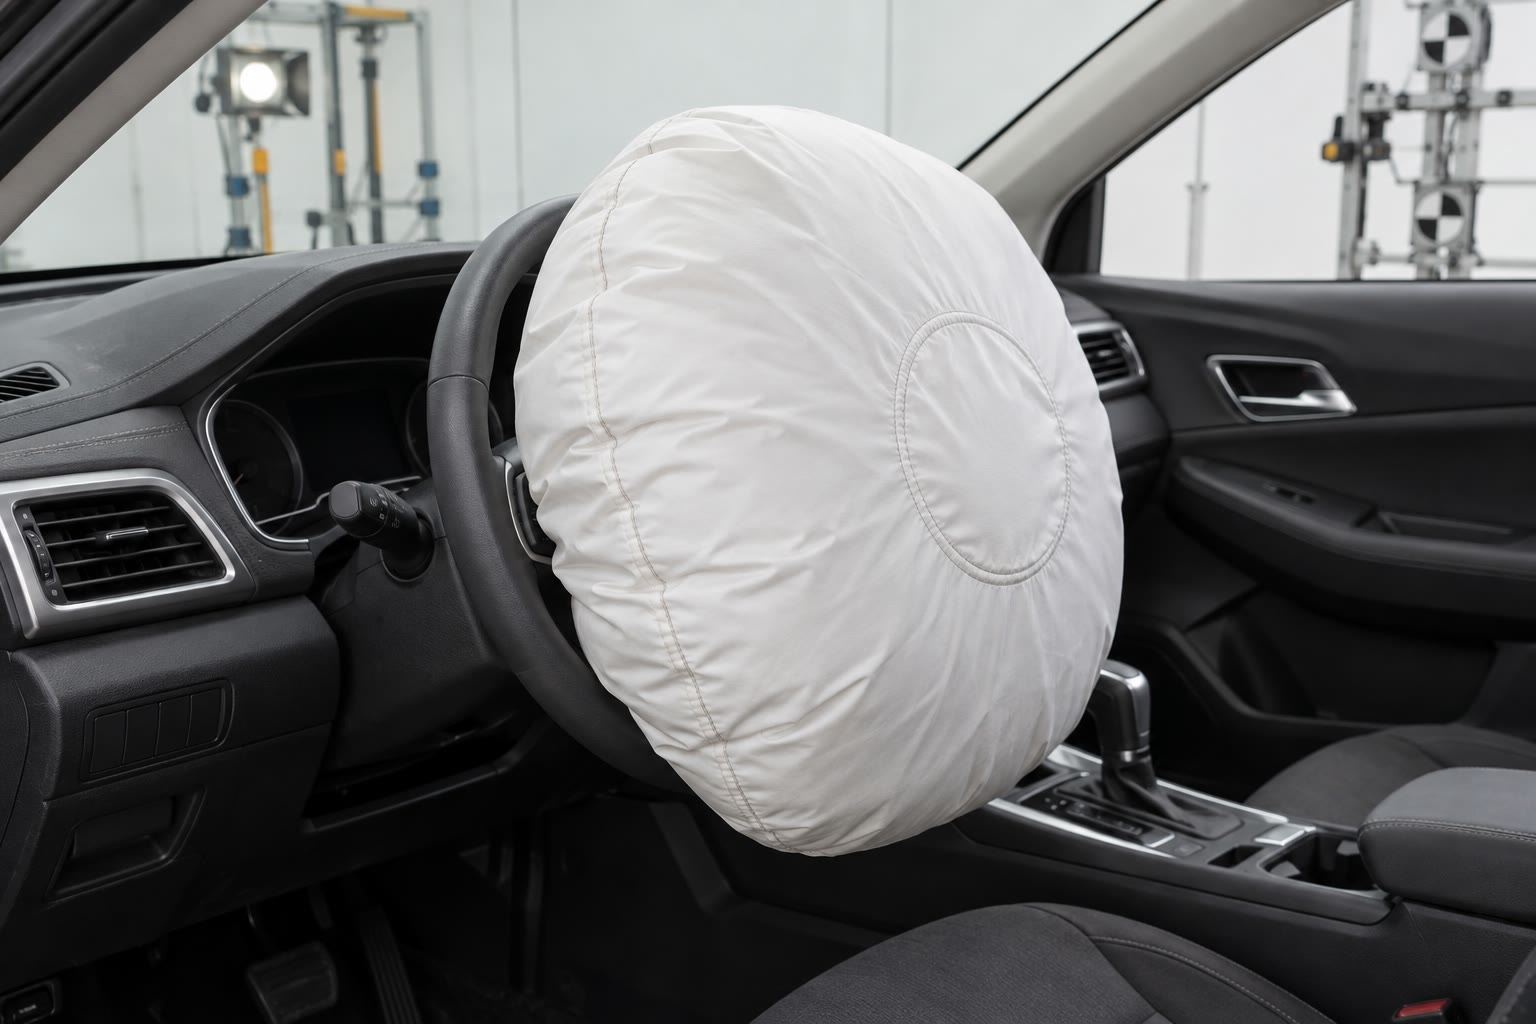
\includegraphics[width=0.5\linewidth]{images/book1/ai/g10-airbag.jpg}

{\small Um airbag se enche numa fração de segundo, com o nitrogênio
produzido por uma reação.}
\end{omfigure}

\section{Descrever um sistema químico}

\begin{definition}[Sistema químico, estados inicial e final]\label{def:g10:reaction-progress-table:system}
Um \emph{sistema químico}\index{sistema quimico@sistema químico} é o conjunto das
\omterm{def:g6:pure-substances-and-mixtures:species}{espécies químicas} presentes num dado lugar (um frasco, uma almofada,
uma pilha), cada uma com a sua \omterm{def:g10:the-mole:amount}{quantidade de matéria} e o seu estado
físico. O sistema antes de a reação começar é o \emph{estado
inicial}\index{estado inicial}; o sistema depois que a reação parou é o
\emph{estado final}\index{estado final}.
\end{definition}


\begin{example}[O metano queimando num recipiente fechado]\label{ex:g10:reaction-progress-table:methane}
Um recipiente fechado contém \qty{2.0}{mol} de metano e \qty{3.0}{mol} de
gás oxigênio; uma faísca desencadeia a \omterm{def:g4:what-a-fire-needs:burning}{combustão}
\ce{CH4 + 2O2 -> CO2 + 2H2O}. No \omterm{def:g10:reaction-progress-table:system}{estado inicial}, o sistema contém
\qty{2.0}{mol} de \ce{CH4(g)}, \qty{3.0}{mol} de \ce{O2(g)} e nenhum
produto. O que há no \omterm{def:g10:reaction-progress-table:system}{estado final}? O resto do capítulo responde.
\end{example}

\section{O avanço da reação e a tabela de avanço}

\begin{definition}[Avanço da reação, tabela de avanço]\label{def:g10:reaction-progress-table:extent}
O \emph{avanço da reação}\index{avanco da reacao@avanço da reação} $x$, em \omterm{def:g10:the-mole:amount}{mols}, conta
quantas vezes a reação, tal como está escrita na \omterm{def:g8:balanced-equations:equation}{equação balanceada},
aconteceu: quando o avanço é $x$, uma espécie de coeficiente $\nu$ foi
consumida (\omterm{def:g7:chemical-reactions:reactant}{reagente}) ou formada (produto) na quantidade $\nu x$. A
\emph{tabela de avanço}\index{tabela de avanco@tabela de avanço} dá, embaixo da equação, a
\omterm{def:g10:the-mole:amount}{quantidade de matéria} de cada espécie no \omterm{def:g10:reaction-progress-table:system}{estado inicial}, num avanço $x$
e no \omterm{def:g10:reaction-progress-table:system}{estado final}.
\end{definition}

\begin{method}[Preencher uma tabela de avanço]\label{met:g10:reaction-progress-table:fill}
\begin{enumerate}
  \item Escreva a \omterm{def:g8:balanced-equations:equation}{equação balanceada} na primeira linha.
  \item \omterm{def:g10:reaction-progress-table:system}{Estado inicial} ($x = 0$): escreva embaixo dela a quantidade
        inicial de cada espécie.
  \item Estado intermediário (avanço $x$): cada \omterm{def:g7:chemical-reactions:reactant}{reagente} de coeficiente
        $\nu$ passa a $n_0 - \nu x$, cada produto a $n_0 + \nu x$.
  \item \omterm{def:g10:reaction-progress-table:system}{Estado final}: encontre $x_{\max}$ (próxima seção) e coloque-o nas
        expressões da linha intermediária.
\end{enumerate}
\end{method}
\begin{omfigure}
\renewcommand{\arraystretch}{1.25}
\begin{tabular}{l|c|cccc}
\hline
equação & & \ce{CH4} & $+$ \ce{2O2} & $\longrightarrow$ \ce{CO2} & $+$ \ce{2H2O} \\
\hline
estado & avanço (\si{mol}) & \multicolumn{4}{c}{quantidades (\si{mol})} \\
\hline
inicial & $0$ & $2.0$ & $3.0$ & $0$ & $0$ \\
intermediário & $x$ & $2.0 - x$ & $3.0 - 2x$ & $x$ & $2x$ \\
final & $x_{\max} = 1.5$ & $0.5$ & $0$ & $1.5$ & $3.0$ \\
\hline
\end{tabular}\par\medskip

{\small A \omterm{def:g10:reaction-progress-table:extent}{tabela de avanço} da \omterm{def:g4:what-a-fire-needs:burning}{combustão} do metano do exemplo. Cada coluna
acompanha uma espécie; os coeficientes 2 do \ce{O2} e da \ce{H2O} viram
o $2x$.}
\end{omfigure}

\section{O reagente limitante e o estado final}

\begin{definition}[Reagente limitante, avanço máximo, reação total]\label{def:g10:reaction-progress-table:limiting}
Uma reação é uma \emph{reação total}\index{reacao total@reação total} se ela só para
quando um dos seus \omterm{def:g7:chemical-reactions:reactant}{reagentes} se esgota. Esse \omterm{def:g7:chemical-reactions:reactant}{reagente} é o
\emph{reagente limitante}\index{reagente limitante}; os outros \omterm{def:g7:chemical-reactions:reactant}{reagentes}
estão em excesso. O avanço em que o \omterm{def:g7:chemical-reactions:reactant}{reagente} limitante se esgota é o
\emph{avanço máximo}\index{avanco maximo@avanço máximo} $x_{\max}$; o \omterm{def:g10:reaction-progress-table:system}{estado final} de
uma reação total é o estado em $x = x_{\max}$.
\end{definition}

\begin{method}[Encontrar o reagente limitante]\label{met:g10:reaction-progress-table:limiting}
\begin{enumerate}
  \item Para cada \omterm{def:g7:chemical-reactions:reactant}{reagente}, resolva $n_0 - \nu x = 0$: o \omterm{def:g7:chemical-reactions:reactant}{reagente} se
        esgotaria em $x = n_0 / \nu$.
  \item O menor desses valores é $x_{\max}$; o \omterm{def:g7:chemical-reactions:reactant}{reagente} que o dá é o
        \omterm{def:g10:reaction-progress-table:limiting}{reagente limitante}.
  \item Coloque $x_{\max}$ na linha intermediária para obter o \omterm{def:g10:reaction-progress-table:system}{estado
        final}; verifique que nenhuma quantidade é negativa.
\end{enumerate}
\end{method}

\begin{example}[De volta ao metano]\label{ex:g10:reaction-progress-table:methane-final}
O metano se esgotaria em $x = 2.0/1 = \qty{2.0}{mol}$, o gás oxigênio em
$x = 3.0/2 = \qty{1.5}{mol}$. O menor é \qty{1.5}{mol}: o gás oxigênio é
o \omterm{def:g10:reaction-progress-table:limiting}{reagente limitante} e $x_{\max} = \qty{1.5}{mol}$. O \omterm{def:g10:reaction-progress-table:system}{estado final}
contém \qty{0.5}{mol} de metano que sobrou, nenhum gás oxigênio,
\qty{1.5}{mol} de dióxido de carbono e \qty{3.0}{mol} de água.
\end{example}

\begin{omfigure}
\begin{tikzpicture}
\begin{axis}[width=0.78\linewidth, height=6.2cm, xmin=0, xmax=2.05,
    ymin=0, ymax=4.2, xlabel={avanço $x$ (\si{mol})},
    ylabel={quantidade (\si{mol})}, axis lines*=left, ymajorgrids,
    grid style={gray!20}, tick label style={font=\small},
    label style={font=\small}, xtick={0,0.5,1,1.5,2},
    legend style={font=\small, at={(1.02,0.5)}, anchor=west, draw=none},
    legend cell align=left]
  \addplot[very thick, omDef, domain=0:2] {2-x};
  \addplot[very thick, omThm, domain=0:1.5] {3-2*x};
  \addplot[very thick, omMeth, domain=0:2] {x};
  \addplot[very thick, omProp, domain=0:2] {2*x};
  \legend{\ce{CH4}, \ce{O2}, \ce{CO2}, \ce{H2O}}
  \addplot[dashed, black!60] coordinates {(1.5,0) (1.5,4.2)};
  \node[font=\small, anchor=south west] at (axis cs:1.5,3.55) {$x_{\max}$};
  \fill[black!8, opacity=0.6] (axis cs:1.5,0) rectangle (axis cs:2.05,4.2);
\end{axis}
\end{tikzpicture}

{\small As quantidades em função do avanço, para o exemplo do metano. O
gás oxigênio (vermelho) chega a zero primeiro, em $x = \qty{1.5}{mol}$:
a reação para ali, e a parte sombreada nunca é alcançada.}
\end{omfigure}

\begin{remark}[Nem todas as reações são totais]\label{rem:g10:reaction-progress-table:not-total}
Muitas reações param antes que algum \omterm{def:g7:chemical-reactions:reactant}{reagente} se esgote: elas chegam a
um estado em que \omterm{def:g7:chemical-reactions:reactant}{reagentes} e produtos coexistem. O seu \omterm{def:g10:reaction-progress-table:system}{estado final} não
é $x_{\max}$, e um capítulo mais adiante ensina a encontrá-lo. Neste
capítulo, todas as reações são totais.
\end{remark}

\section{A mistura estequiométrica}

\begin{definition}[Mistura estequiométrica]\label{def:g10:reaction-progress-table:stoichiometric}
Uma \omterm{def:g6:pure-substances-and-mixtures:mixture}{mistura} de \omterm{def:g7:chemical-reactions:reactant}{reagentes} é uma \emph{mistura
estequiométrica}\index{mistura estequiometrica@mistura estequiométrica} quando as quantidades
iniciais estão nas proporções dos coeficientes da \omterm{def:g8:balanced-equations:equation}{equação balanceada}.
\end{definition}

\begin{proposition}[Todos os reagentes se esgotam juntos]\label{prop:g10:reaction-progress-table:together}
Para uma reação $a\,\ce{A} + b\,\ce{B} \longrightarrow$ produtos, a \omterm{def:g6:pure-substances-and-mixtures:mixture}{mistura} é estequiométrica se
e somente se
\[
  \frac{n_0(\ce{A})}{a} = \frac{n_0(\ce{B})}{b},
\]
e então, para uma \omterm{def:g10:reaction-progress-table:limiting}{reação total}, os dois \omterm{def:g7:chemical-reactions:reactant}{reagentes} estão consumidos no
\omterm{def:g10:reaction-progress-table:system}{estado final}.
\end{proposition}

\begin{proof}
\ce{A} se esgotaria em $x = n_0(\ce{A})/a$, \ce{B} em $x = n_0(\ce{B})/b$.
Os dois valores são iguais exatamente quando as proporções são as da
equação, e então o avanço $x_{\max}$ esvazia os dois de uma vez.
\end{proof}

\begin{example}[Queimar o metano de forma limpa]\label{ex:g10:reaction-progress-table:stoich}
Para \ce{CH4 + 2O2 -> CO2 + 2H2O}, \qty{2.0}{mol} de metano precisam de
\qty{4.0}{mol} de gás oxigênio: $2.0/1 = 4.0/2$. Com só \qty{3.0}{mol}
de gás oxigênio, a \omterm{def:g6:pure-substances-and-mixtures:mixture}{mistura} do primeiro exemplo tinha falta de oxigênio;
numa chama real, essa falta é o que produz o venenoso monóxido de
carbono (\cref{ch:g8:combustion-and-fuels}).
\end{example}

\section{Gases e soluções na tabela}


\begin{method}[As quantidades do estado inicial]\label{met:g10:reaction-progress-table:amounts}
Antes de preencher uma tabela, converta cada grandeza dada numa
\omterm{def:g10:the-mole:amount}{quantidade de matéria}: $n = m/M$ para um sólido ou um líquido pesado;
$n = V/V_m$ para um gás; $n = c \times V$ para uma espécie dissolvida.
No fim, converta de volta as quantidades do \omterm{def:g10:reaction-progress-table:system}{estado final} no que for
pedido: massa, volume de gás ou concentração.
\end{method}

\begin{example}[O magnésio no ácido clorídrico]\label{ex:g10:reaction-progress-table:magnesium}
% ledger: aw:Mg
O ácido clorídrico contém \omterm{def:g9:ions:ion}{íons} hidrogênio \ce{H+}, que atacam o magnésio:
\ce{Mg + 2H+ -> Mg^{2+} + H2}. Uma fita de \qty{0.12}{g} de magnésio é
colocada em \qty{50.0}{mL} de ácido com $c(\ce{H+}) = \qty{1.0}{mol/L}$.
Quantidades iniciais: $n_0(\ce{Mg}) = 0.12/24.3 = \qty{4.9e-3}{mol}$ e
$n_0(\ce{H+}) = 1.0 \times 0.0500 = \qty{5.0e-2}{mol}$. O magnésio se
esgotaria em $x = \qty{4.9e-3}{mol}$, os \omterm{def:g9:ions:ion}{íons} hidrogênio em
$x = 0.050/2 = \qty{2.5e-2}{mol}$: o magnésio é limitante e
$x_{\max} = \qty{4.9e-3}{mol}$. A reação dá \qty{4.9e-3}{mol} de gás
hidrogênio, isto é, $\num{4.9e-3} \times 24.1 = \qty{0.12}{L}$ a
\qty{20}{\celsius}, e deixa $0.050 - 2 \times 0.0049 =
\qty{0.040}{mol}$ de \omterm{def:g9:ions:ion}{íons} hidrogênio em excesso.
\end{example}

\begin{inthelab}[Balões nos frascos]
O professor despeja \qty{50.0}{mL} do mesmo ácido clorídrico em cada um
de seis erlenmeyers, e coloca em seis balões massas crescentes de
magnésio em pó: 0.15, 0.30, 0.45, 0.60, 0.75 e \qty{0.90}{g}. Cada balão
é encaixado no gargalo do seu frasco e depois levantado, para que o pó
caia no ácido. Borbulhando, os balões incham. Quando tudo para, os balões
são cada vez maiores do primeiro frasco até o quarto; o quarto, o quinto
e o sexto têm o mesmo tamanho, e nos dois últimos sobra um pó cinza no
fundo do frasco.
\end{inthelab}

\begin{omfigure}
\begin{tikzpicture}[font=\small, scale=0.82]
  % H2 volume (L): 0.149 0.298 0.446 0.595 0.6025 0.6025; radius ~ V^(1/3)
  \foreach \i/\m/\v/\r/\left in {0/0.15/0.15/0.42/0, 1/0.30/0.30/0.53/0,
      2/0.45/0.45/0.61/0, 3/0.60/0.60/0.67/0, 4/0.75/0.60/0.67/1,
      5/0.90/0.60/0.67/1} {
    \begin{scope}[shift={(2.35*\i,0)}]
      \pic[transform shape] at (0,0) {erlenmeyer={0.25}{omWater}};
      \ifnum\left=1
        \fill[black!45] (-0.5,0.03) rectangle (0.5,0.12);
      \fi
      \fill[omProp!35, draw=omProp!80!black] (-0.3,2.6) -- (0.3,2.6)
        -- (0.12,2.82) -- (-0.12,2.82) -- cycle;
      \shade[ball color=omProp!40, draw=omProp!80!black]
        (0,{2.78+\r}) circle (\r);
      \node[align=center, anchor=north] at (0,-0.15)
        {\qty{\m}{g} Mg\\ \qty{\v}{L}};
    \end{scope}
  }
\end{tikzpicture}

{\small Seis frascos com o mesmo ácido e massas crescentes de magnésio,
com o volume de gás hidrogênio (a \qty{20}{\celsius}) em cada balão.
Acima de cerca de \qty{0.61}{g}, o ácido é limitante: os balões param de
crescer e sobra magnésio (cinza).}
\end{omfigure}

\begin{remark}[Ler o patamar]\label{rem:g10:reaction-progress-table:plateau}
Nos primeiros frascos, o magnésio é o \omterm{def:g10:reaction-progress-table:limiting}{reagente limitante}, e dobrá-lo
dobra o gás. A partir de uma certa massa, os \omterm{def:g9:ions:ion}{íons} hidrogênio se esgotam
primeiro: acrescentar magnésio não muda nada além do pó que sobra. A
mudança acontece exatamente na \omterm{def:g10:reaction-progress-table:stoichiometric}{mistura estequiométrica},
$n_0(\ce{Mg}) = n_0(\ce{H+})/2 = \qty{0.025}{mol}$, isto é,
$0.025 \times 24.3 = \qty{0.61}{g}$ de magnésio.
\end{remark}

\begin{safety}{\ghs[0.82cm]{GHS02}\ghs[0.82cm]{GHS05}\ghs[0.82cm]{GHS07}}
% ledger: ghs:Mg, ghs:HCl
O magnésio em pó é inflamável; o ácido clorídrico queima a pele e os
olhos e os seus vapores irritam as vias respiratórias; o gás hidrogênio
\omterm{def:g4:what-a-fire-needs:burning}{queima} no \omterm{def:g4:air-a-mixture-of-gases:air}{ar}. Uma demonstração feita pelo professor, com óculos de
proteção, longe de qualquer chama.
\end{safety}

\section{Exercícios}

\begin{exercise}[$\star$]\label{exo:g10:reaction-progress-table:1}
Preencha a \omterm{def:g10:reaction-progress-table:extent}{tabela de avanço} de \ce{2H2 + O2 -> 2H2O} para uma \omterm{def:g6:pure-substances-and-mixtures:mixture}{mistura}
inicial de \qty{4.0}{mol} de gás hidrogênio e \qty{3.0}{mol} de gás
oxigênio, supondo a \omterm{def:g10:reaction-progress-table:limiting}{reação total}. Dê $x_{\max}$, o \omterm{def:g10:reaction-progress-table:limiting}{reagente limitante} e
o \omterm{def:g10:reaction-progress-table:system}{estado final}.
\end{exercise}

\begin{exercise}[$\star$]\label{exo:g10:reaction-progress-table:2}
O carbono \omterm{def:g4:what-a-fire-needs:burning}{queima} no gás oxigênio: \ce{C + O2 -> CO2}. Partindo de
\qty{3.0}{mol} de carbono e \qty{2.0}{mol} de gás oxigênio, encontre
$x_{\max}$, o \omterm{def:g10:reaction-progress-table:limiting}{reagente limitante} e o \omterm{def:g10:reaction-progress-table:system}{estado final}.
\end{exercise}

\begin{exercise}[$\star$]\label{exo:g10:reaction-progress-table:3}
O ferro e o enxofre reagem quando aquecidos: \ce{Fe + S -> FeS}.
Partindo de \qty{0.50}{mol} de ferro e \qty{0.30}{mol} de enxofre,
descreva o \omterm{def:g10:reaction-progress-table:system}{estado final}.
\end{exercise}

\begin{exercise}[$\star$]\label{exo:g10:reaction-progress-table:4}
Suponha que a reação \ce{N2 + 3H2 -> 2NH3} seja total. Partindo de
\qty{1.0}{mol} de gás nitrogênio e \qty{2.4}{mol} de gás hidrogênio,
encontre $x_{\max}$ e o \omterm{def:g10:reaction-progress-table:system}{estado final}.
\end{exercise}

\begin{exercise}[$\star$]\label{exo:g10:reaction-progress-table:5}
Para \ce{2CO + O2 -> 2CO2}, qual destas \omterm{def:g6:pure-substances-and-mixtures:mixture}{misturas} é estequiométrica?
(a) \qty{2}{mol} de \ce{CO} e \qty{2}{mol} de \ce{O2}; (b) \qty{4}{mol}
de \ce{CO} e \qty{2}{mol} de \ce{O2}; (c) \qty{1}{mol} de \ce{CO} e
\qty{2}{mol} de \ce{O2}.
\end{exercise}

\begin{exercise}[$\star\star$]\label{exo:g10:reaction-progress-table:6}
Que massa de gás oxigênio é necessária para queimar completamente
\qty{32}{g} de metano (\ce{CH4 + 2O2 -> CO2 + 2H2O})? Que massa de água
é formada?
\end{exercise}

\begin{exercise}[$\star\star$]\label{exo:g10:reaction-progress-table:7}
Um fogareiro de camping \omterm{def:g4:what-a-fire-needs:burning}{queima} \qty{1.0}{kg} de propano:
\ce{C3H8 + 5O2 -> 3CO2 + 4H2O}. Que volume de dióxido de carbono, a
\qty{20}{\celsius}, ele libera?
\end{exercise}

\begin{exercise}[$\star\star$]\label{exo:g10:reaction-progress-table:8}
Usando a figura das quantidades em função do avanço para o exemplo do
metano, leia as quantidades das quatro espécies em $x = \qty{1.0}{mol}$.
Por que a linha do gás oxigênio para em $x = \qty{1.5}{mol}$?
\end{exercise}

\begin{exercise}[$\star\star$]\label{exo:g10:reaction-progress-table:9}
Acrescentam-se \qty{1.30}{g} de zinco em pó a \qty{100.0}{mL} de uma
solução azul de sulfato de cobre a \qty{0.10}{mol/L}. A reação é
\ce{Zn + Cu^{2+} -> Zn^{2+} + Cu}.
Encontre o \omterm{def:g10:reaction-progress-table:limiting}{reagente limitante}, a massa de cobre formada e a massa de
zinco que sobra. A solução continua azul no fim?
\end{exercise}

\begin{exercise}[$\star\star$]\label{exo:g10:reaction-progress-table:10}
Acrescentam-se \qty{0.48}{g} de magnésio a \qty{20.0}{mL} de ácido
clorídrico com $c(\ce{H+}) = \qty{1.0}{mol/L}$
(\ce{Mg + 2H+ -> Mg^{2+} + H2}). Que \omterm{def:g7:chemical-reactions:reactant}{reagente} é limitante? Que volume de
gás hidrogênio é recolhido a \qty{20}{\celsius}?
\end{exercise}

\begin{exercise}[$\star\star$]\label{exo:g10:reaction-progress-table:11}
No exercício~3, em que porcentagem o \omterm{def:g7:chemical-reactions:reactant}{reagente} em excesso ultrapassa a
quantidade que teria formado uma \omterm{def:g10:reaction-progress-table:stoichiometric}{mistura estequiométrica}?
\end{exercise}

\begin{exercise}[$\star\star\star$]\label{exo:g10:reaction-progress-table:12}
Um aluno quer \qty{10.0}{g} de uma \omterm{def:g10:reaction-progress-table:stoichiometric}{mistura estequiométrica} de ferro e
enxofre para \ce{Fe + S -> FeS}. Que massas de ferro e de enxofre ele
deve pesar?
\end{exercise}

\begin{exercise}[$\star\star\star$]\label{exo:g10:reaction-progress-table:13}
\qty{10.0}{g} de calcário \ce{CaCO3} são fortemente aquecidos e se
decompõem totalmente: \ce{CaCO3 -> CaO + CO2}. A cal virgem \ce{CaO}
obtida é depois colocada em \qty{1.8}{g} de água:
\ce{CaO + H2O -> Ca(OH)2}.
\begin{enumerate}
  \item Preencha a \omterm{def:g10:reaction-progress-table:extent}{tabela de avanço} da primeira reação; que volume de
        dióxido de carbono é liberado a \qty{20}{\celsius}?
  \item Preencha a tabela da segunda reação. Que \omterm{def:g7:chemical-reactions:reactant}{reagente} é limitante?
        Que massa de cal hidratada \ce{Ca(OH)2} é formada?
\end{enumerate}
\end{exercise}

\begin{exercise}[$\star\star\star$]\label{exo:g10:reaction-progress-table:14}
No experimento dos balões do quadro de laboratório, calcule o volume de
gás hidrogênio em cada balão. Explique por que ele para de crescer depois
do quarto frasco, e trace (à mão) o volume de gás em função da massa de
magnésio.
\end{exercise}

\begin{exercise}[$\star\star\star$]\label{exo:g10:reaction-progress-table:15}
\qty{4.6}{g} de etanol \ce{C2H6O} queimam num recipiente fechado que
contém \qty{4.8}{L} de gás oxigênio a \qty{20}{\celsius}:
\ce{C2H6O + 3O2 -> 2CO2 + 3H2O}. Encontre o \omterm{def:g10:reaction-progress-table:limiting}{reagente limitante}, a massa
de etanol que sobra sem queimar e o volume de dióxido de carbono
formado.
\end{exercise}

\section{Problema: o airbag}

\begin{problem}[{Problema de fim de semana --- que massa de azida de
sódio deve ser colocada num volante para encher um airbag de 60
litros?}]
\label{pb:g10:reaction-progress-table:1}
% ledger: use:NaN3-airbag, ghs:NaN3, aw:Na, aw:N, aw:K, aw:O
No modelo clássico de airbag, uma faísca elétrica desencadeia a
decomposição da azida de sódio sólida:
\[
  \ce{2NaN3 -> 2Na + 3N2} .
\]
O sódio metálico formado é perigoso: ele reage violentamente com a água,
e com a umidade da pele e dos olhos. Por isso, a carga também contém
nitrato de potássio, que transforma o sódio em óxidos inofensivos e dá
um pouco mais de nitrogênio:
\[
  \ce{10Na + 2KNO3 -> K2O + 5Na2O + N2} .
\]
As duas reações são totais. O airbag deve ser enchido com \qty{60}{L} de
nitrogênio; tome o gás a \qty{20}{\celsius}, onde
$V_m = \qty{24.1}{L/mol}$.

\medskip
\noindent\textbf{Parte I --- As reações.}
\begin{enumerate}
  \item Verifique que a primeira equação está balanceada, elemento por
        elemento.
  \item Verifique que a segunda equação está balanceada.
  \item Que capítulo anterior mostrou que o sódio reage violentamente com
        a água? Por que nenhum sódio pode sobrar depois da batida?
  \item Calcule as \omterm{def:g10:the-mole:molar-mass}{massas molares} da azida de sódio \ce{NaN3} e do
        nitrato de potássio \ce{KNO3}.
\end{enumerate}

\medskip
\noindent\textbf{Parte II --- A decomposição.}
\begin{enumerate}[resume]
  \item Preencha a \omterm{def:g10:reaction-progress-table:extent}{tabela de avanço} da primeira reação para uma
        quantidade inicial de \qty{1.00}{mol} de azida de sódio.
  \item Encontre $x_{\max}$. Qual é o \omterm{def:g10:reaction-progress-table:limiting}{reagente limitante}?
  \item Dê as quantidades de sódio e de nitrogênio no \omterm{def:g10:reaction-progress-table:system}{estado final}.
  \item Que volume de nitrogênio \qty{1.00}{mol} de azida de sódio dá a
        \qty{20}{\celsius}?
\end{enumerate}

\medskip
\noindent\textbf{Parte III --- Eliminar o sódio.}
\begin{enumerate}[resume]
  \item Preencha a \omterm{def:g10:reaction-progress-table:extent}{tabela de avanço} da segunda reação, partindo do sódio
        encontrado na questão 7 e de uma quantidade $n$ de nitrato de
        potássio.
  \item Que quantidade, e que massa, de nitrato de potássio forma uma
        \omterm{def:g10:reaction-progress-table:stoichiometric}{mistura estequiométrica} com esse sódio?
  \item Dê o \omterm{def:g10:reaction-progress-table:system}{estado final} da segunda reação para essa \omterm{def:g6:pure-substances-and-mixtures:mixture}{mistura}.
  \item Se só fossem colocados \qty{0.150}{mol} de nitrato de potássio,
        que \omterm{def:g7:chemical-reactions:reactant}{reagente} seria limitante, e o que sobraria? Por que isso
        seria perigoso?
\end{enumerate}

\medskip
\noindent\textbf{Parte IV --- O airbag de 60 litros.}
\begin{enumerate}[resume]
  \item Pelas questões 7 e 11, que quantidade de nitrogênio a carga
        inteira dá por \omterm{def:g10:the-mole:amount}{mol} de azida de sódio?
  \item Que quantidade de nitrogênio enche o airbag?
  \item Deduza a quantidade de azida de sódio necessária.
  \item Calcule a sua massa.
  \item Calcule a massa de nitrato de potássio a acrescentar.
  \item Sem a segunda reação, que massa de azida de sódio teria sido
        necessária? Quanto a segunda reação economiza?
  \item A azida de sódio é mortal se ingerida. Por que importa que a
        primeira reação seja total, e como a \omterm{def:g10:reaction-progress-table:extent}{tabela de avanço} mostra que
        não sobra nenhuma?
  \item Dê a resposta final: que massa de azida de sódio enche um airbag
        de \qty{60}{L}?
\end{enumerate}
\end{problem}
